%%% ====================================================================
%%% Início da parte textual do documento.


%%% Configuração do espaçamento entre títulos e texto
\setlength{\afterchapskip}{1.5cm minus \baselineskip}


\chapter{Introdução}
\label{cha:introducao}
Em um contexto onde a quantidade e disponibilidade de informações vem sendo cada vez maior, as pessoas vem se deparando com uma enorme diversidade de opções \cite{cazella2010}. Deste modo, o excesso de informação, muitas vezes, acaba tornando o processo de tomada de decisão mais complexo para o utilizador \cite{centeno2018}.

Como uma alternativa ao problema levantado, têm-se os sistemas de recomendação, que, segundo \citeonline{cazella2010}, podem ser definidos como um sistema que a partir de dados recomendados por usuários, consegue agregar e direcionar a recomendação gerada para os potenciais indivíduos interessados nelas.

Segundo estudos de \citeonline{pathak2010}, a utilização de sistemas de recomendação de produtos pode acabar gerando aumento nas vendas e lucratividade em diversos setores como o comércio eletrônico, fazendo com que a utilização desses sistemas gere vantagem competitiva para seus utilizadores. Como exemplo de sucesso nesse setor, pode-se citar a Amazon, que como apresentado nos trabalhos de \citeonline{smith2017}, vem utilizando algoritmos de recomendação há mais de duas décadas.

Outro exemplo de sucesso na utilização de sistemas de recomendação pode ser visto no Youtube, que em sua página inicial (gerada a partir de sistemas de recomendação) consegue uma taxa de assertividade (vídeos visualizados) em torno de 60\% na recomendação de vídeos a partir da análise do perfil e das preferências de seus usuários \cite{davidson2010youtube}.

O uso de sistemas de recomendação também ocorre em diversas outras áreas, como na educação por exemplo, onde a utilização de recomendações pode auxiliar no desenvolvimento de sistemas educacionais mais eficazes \cite{costa2013sistemas}. Um exemplo de uso da recomendação nesses sistemas pode ocorrer a partir da seleção de conteúdos baseados nas preferências e características de cada indivíduo \cite{adomavicius2005}. 

Áreas como a da saúde também podem ser beneficiadas, uma vez que a utilização desses sistemas pode auxiliar na identificação de fatores e problemas relacionados a saúde, como defendido por \citeonline{weitzel2010sistemas}, podendo até mesmo identificar e utilizar perfis e características do paciente para realizar a recomendação.

Além disso, na última década, é visto um crescente aumento na busca do termo \textit{Recommendation system}, como demonstrado na Figura \ref{fig:googletrends}, o que reflete a relevância dessa área nos dias atuais.

\begin{figure}[H]
	\centering
	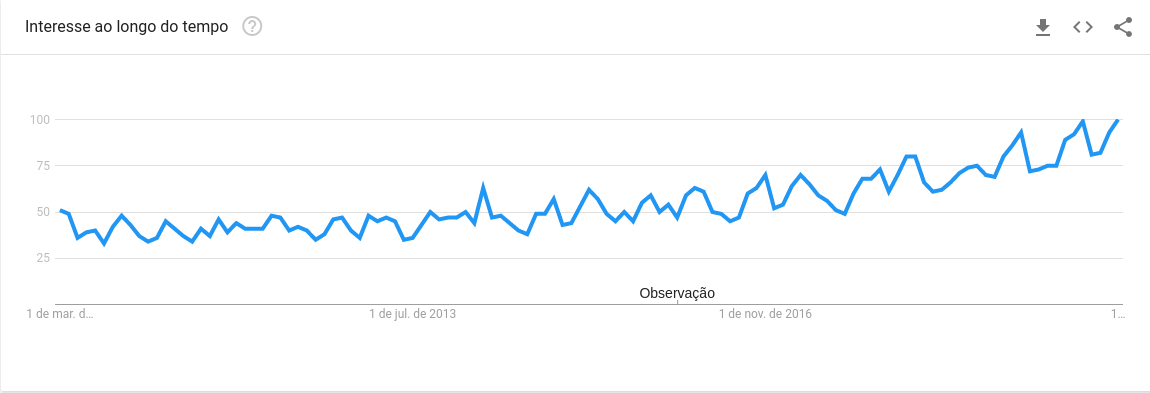
\includegraphics[width=1\linewidth]{imagens/googletrends.png}
	\caption[Número de buscas do termo recommendation system]{Número de buscas do termo "recommendation system" no Google Trends}
	\label{fig:googletrends}
\end{figure}

\nocite{googletrends}